% To keep the analysis simple, we initially ignore transaction costs. 
% We modify the basic framework to include these costs and consider how it changes the results. 
% One of the main findings is that when transactions costs are sufficiently high, the P2P rental market cannot exist. 
% This finding suggests that the technological changes---namely the maturation and increasing penetration of the Internet and web-based technologies---were the technological shock that made these P2P rental markets feasible. 

In practice, the utilization of a good---even with an efficient P2P rental market---will be far less than 100\%.
Setting up trades, making repairs, transporting goods and so on all take time.  
Furthermore, even durable goods are consumed more quickly when used more intensively. 
There are several ways one could model these kinds of practicalities. 

For utilization, one modeling approach is to simply re-define what is the unit of time available and the corresponding $\alpha$. 
For example, we might think of a the unit of time for a vacation home on a ski slope to be 4 months, with high-types wanting to take three week vacations and low-types one week vacations and one week in total lost to cleaning and maintenance.      
For transaction costs, we could think of owners in the P2P rental market as facing a cost of $c$ that captures both the transaction costs of listing on a market, finding trading partners and so on, as well as the cost from increased usage that leads to either more extensive or more frequent repairs or faster replacement.
In the short-run P2P equilibrium, $c$ provides a price-floor in the rental market.  
In the long-run P2P equilibrium, the rental rate ``includes'' these costs, with $r_{LR} = p + c$. 

If $c$ is sufficiently high, then no P2P rental market will exist in either the short- or long-run: 
many goods have ``missing'' rental markets because the rental rate $r$ required to cover the added transaction costs of renting would be prohibitive.
Goods that have unpredictable usage patterns would be particularly poor rental candidates.  
It is only with the emergence of computer-mediated platforms that seem to dramatically reduce transaction costs that a P2P rental market has emerged for some of these goods. 
Before these markets sprung up, simply finding an appropriate trading partner would be difficult, to say nothing of coming to terms, writing a contract, monitoring compliance, handling disputes, making payment and so on. 



Monitoring usage 

\subsection{The incidence of transaction costs}
The per-unit cost $\gamma$ effectively functions like an ad valorem tax in the P2P rental market.
The natural question is the incidence of these bringing-to-market costs.\footnote{
 This issue has become a matter of public policy interest, as Uber faces a class action lawsuit by drivers seeking reimbursement for some of their costs such as car depreciation and fuel. 
}
The short-run elasticity of demand is

While we assume that costs are homogeneous across individuals, in practice they surely differ and these differences will likely matter greatly in the low-run in explaining who owns. 
For example, some people enjoy driving, talking to strangers and have a full-time job with fixed and inflexible hours.
For them, driving for Uber is very low cost and may be something close to a hobby (though they still bear gas and depreciation costs).

%In this long-run P2P rental equilibrium, even though both types own, we might expect in that even with the indifference condition, higher-valuation types to be the ones to own, as they can better bear the risk in the rental rate, ala \cite{sinai2005}.

% \section{Continuous Types Model} 
% Assume that $\alpha \sim U[0,1]$. 
% Each consumer---if they consume at all---consumes $x_i = \alpha_i - r/2$. 
% The consumer indifferent between purchasing and not has $\bar{\alpha} = \sqrt{p}$. 
% At a rental rate of $r$, only those with $\alpha > r/2$ consumer any of the good. 
% Let $\underline{\alpha} = r/2$. 
% Short-run market clearing is thus: 
% \begin{align}
% \int_{\underline{\alpha}}^{\bar{\alpha}} x(\alpha, r)\,d\alpha = \int_{\bar{\alpha}}^1 \left( 1 - x(\alpha,r) \right)  \,d\alpha
% \end{align} 
% and so 
% \begin{align} 
% r^* = 2 \left(1-\sqrt{2} \sqrt{1-\sqrt{p}}\right).
% \end{align} 
% For $p \le \frac{1}{4}$, $r^* \le 0$. 

% \begin{figure}
% \centering
% \caption{Comparison of long- and short-run rental rates as a function of market-clearing price} 
% \begin{minipage}{0.80 \linewidth}
% 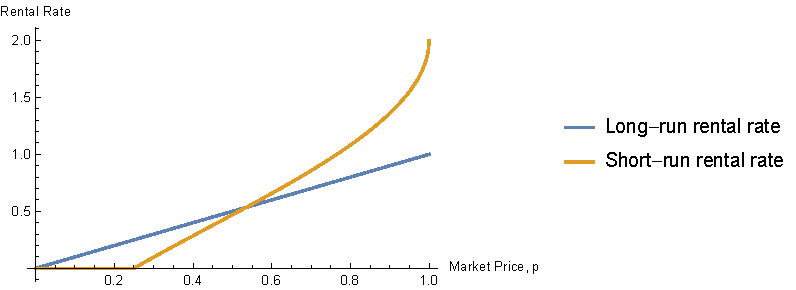
\includegraphics{./plots/cont_types.pdf}
% \end{minipage}
% \end{figure} 

% \begin{figure}
% \centering
% \caption{Quantity exchanged} 
% \begin{minipage}{0.80 \linewidth}
% 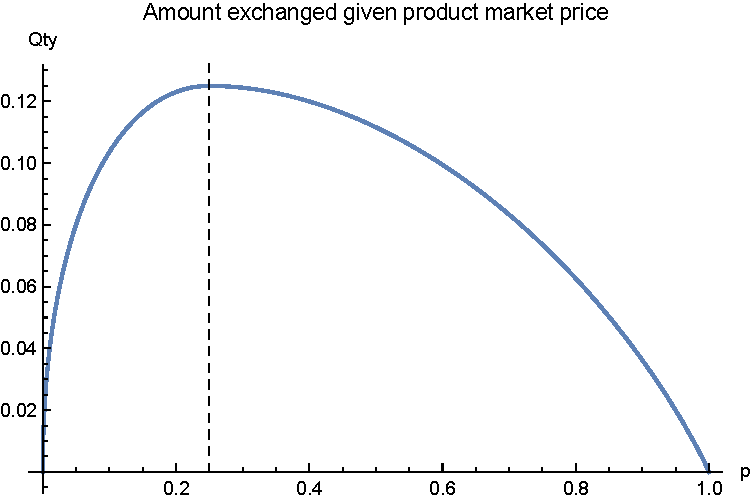
\includegraphics{./plots/cont_qty.pdf}
% \end{minipage}
% \end{figure} 


%% Figure~\ref{fig:welfare} shows a contour plot of change in social surplus from the emergence of the P2P rental market for the space of possible valuation parameters.
%% The figure shows that higher values of $\alpha_L$ increase the gain in social surplus.
%% Indeed, $\partial \Delta S/\partial \alpha_L = 1 - \alpha_H + \alpha_L > 0$ since $\alpha_H < 1$ and $\alpha_L > 0$. 
%% \important{The more the non-owners value the good, the greater the increase in social surplus from the emergence of P2P rental markets.} 
%% The case of $\alpha_H$ is more complex. 
%% Recall that a positive rental rate only occurs when $\alpha_H + \alpha_L > 1$.
%% \important{As such, an increase in the valuation of the high-types reduces social surplus from P2P rental markets in non-glut P2P rental scenarios:   
%% \begin{align} 
%% \frac{\partial \Delta S}{\partial \alpha_H} =  1 - (\alpha_H + \alpha_L) < 0.
%% \end{align}} 
%% In Figure~\ref{fig:welfare} the line stretching from $(1,0)$ to $(1/2, 1/2)$ indicates the glut/non-glut boundary. 
%% For all points to the right of that line, a higher $\alpha_H$ valuation reduces social surplus.  
%% As, such the greatest social surplus is ``unlocked'' by the emergence of the P2P rental market when both purchasers and non-purchasers have similar, high valuations. 
%% In terms of the figure, the highest obtainable social surplus values for a fixed $\alpha_H + \alpha_L$ run along the 45 degree line that indicates $\alpha_H \approx \alpha_L$. 

%% For simplicity, we have ignored income effects as a cause of the pattern of ownership. 
%% However, for goods where income effects are important in the consumer's ownership decision problem, the $\alpha_H > \alpha_L$ requirement would no longer hold and potentially larger gains in social surplus would be unlocked by the P2P rental market emergence. 

%% \begin{figure}
%% \centering 
%% \caption{Consumer welfare as a function of high- and low-type consumer valuations}
%% \label{fig:welfare}
%% \begin{minipage}{0.50 \linewidth}
%% 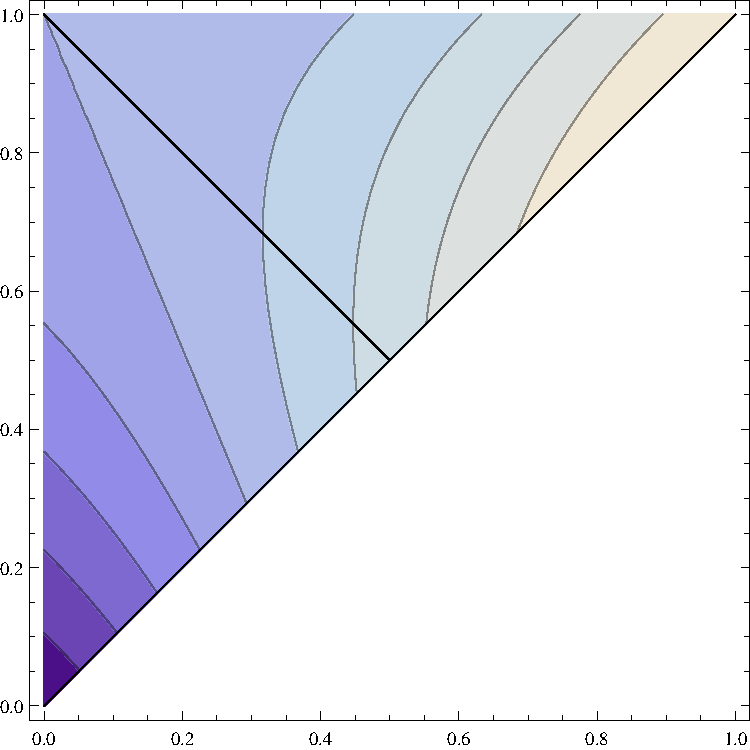
\includegraphics[width = \linewidth]{./plots/welfare.pdf} \\
%% \emph{Notes}: This contour plot shows the level of social surplus created by a P2P rental market at different valuation parameters for the low-type (on the x-axis) and the high-type (on the y-axis).
%% Lighter shading indicates a higher value. 
%% \end{minipage} 
%% \end{figure} 

A cursory look at some certain prices suggest sharing economy platforms with large penetration are having substantial effects:  
the price of NYC taxi medallion has fallen from \$1.3 million in April 2013 to \$840,000 by March 2015---the first observed fall in price for a medallion---and this fall is widely attributed to the rise of Uber (though during this same period outer-borough green taxis were also introduced, so even here, causal claims require care).\footnote{
  \url{http://www.cnbc.com/id/102473287}
}


% grep '\\important{' sharing.tex | sed 's/\\important{//g' | sed 's/}//g'
% Sarah Cannon ; Lawrence Summers
% http://blogs.hbr.org/2014/10/how-uber-and-the-sharing-economy-can-win-over-regulators/
% http://blogs.hbr.org/2013/01/from-zipcar-to-the-sharing-eco/

%% Recent technological advances and entrepreneurial efforts have created a number of new peer-to-peer rental markets in which owners can rent out their durable goods. 
%% We consider the emergence of such a market and determine the market clearing rental rate, the patterns of trade and the surplus unlocked for different types of consumers. 
%% Our analysis considers both a short-run, before consumers can revise their ownership decisions and a long-run, in which they can.
%% We also consider how bringing-to-market costs to affects the analysis. 
%% A survey of consumers finds broad support for the modeling conventions used---namely that ownership is determined by a forward-looking evaluation of planned usage.
%% We also explore the factors that are permitting these new markets to
%% flourish.

% TODO: Better title?
% TODO: Cite to that Slee guy; Dean Baker and the platform cooperative guy for criticisms
% TODO: What are the best insights from the theory model? Emphasize them in the introduction
% TODO: Add citations to the ``factors'' section of the paper
% TODO: Pass through in the BMC short-run - can we say anything about incidence? 
% D[2\left[ (1-\theta)\alpha_L - (1-\alpha_H) \theta \right], \theta] = 2 [1 - (alpha_H - \alpha_L)] + \gamma

%\section{To Cite}

% Model description

% TODO: Add to parts about hard-won industrial experience.

%% Let $r_{SR}$ be the short-run rental rate, which we recall from Equation~\ref{eq:strr} is $2[(1- \theta) \alpha_L - \theta(1 - \alpha_H)]$. 
%% If demand is higher after the long-run P2P equilibrium emerges, then  
%% \begin{align} 
%% D_{1}(p) & > D_{0}(p) \notag \\
%% \theta \alpha_H + (1- \theta) \alpha_L - p/2 &> \theta \notag \\
%% (1- \theta) \alpha_L - \theta(1 - \alpha_H) - p/2 &> 0 \notag \\
%% 2[(1- \theta) \alpha_L - \theta(1 - \alpha_H)] - p &> 0 \notag \\
%% r_{SR}  &> p, 
%% \end{align} 
%% which implies that if the market-clearing short-run rental rate is above the purchase price, ownership will increase in the long-run.
